%------------------------------------------------------------------------------
%Description       : DDMoRe WP7.2.1 First Technical Specification for the Model
%                                   Repository Infrastructure - Proposed Design 
%Author            : Mihai Glonț <mglont@ebi.ac.uk>
%Organization      : EMBL-EBI
%                    Wellcome Trust Genome Campus
%                    Hinxton
%                    Cambridge
%                    United Kingdom
%------------------------------------------------------------------------------
\section{Scenarios}
\label{scenarios}
Having defined the context and the needs of the \ddmore Model Repository, we now proceed to describe the envisaged solution. First, we present a high-level view of the features that will be available. A comprehensive list of scenarios along with low-fidelity designs illustrate how users will interact with the Repository. Next we discuss how the Repository can be accessed programmatically, from other software components. We conclude this section with considerations on the security of an instance of the \ddmore Model Repository as well as the licence requirements. 

\subsection{Use Cases}
\label{useCases}
The aim of this section is to describe how each of the stakeholders from Section~\ref{users} interact with the system. Each such interaction is called a \gls{usecase}, while the user performing it is known as an \gls{actor}. The use cases listed in Figure~\ref{fig:useCases} only consider the main actors that are involved, hence Administrators are not mentioned in any model-related use cases, in spite of the fact that they do have the authority required to perform any action. 

\begin{figure}[htb]
\centering
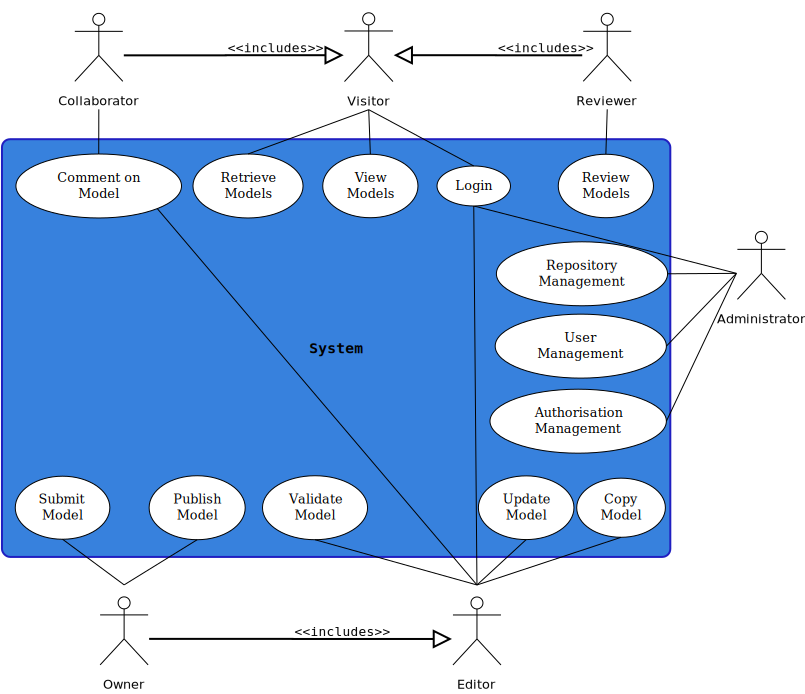
\includegraphics{img/UseCases}
\caption{Diagrammatic representation of the system's scope.}
\label{fig:useCases}
\end{figure}

\subsection{Proposed Work flows}
\label{workFlows}
\idea{Scenarios/Stories go here, along with UML Activity and Sequence diagrams.}

\subsection{Mock-ups}
\label{mockUps}
\idea{General UXD comments behind the look and feel of the pages. Actual mock-ups should be in the appendix. Landscape page format might be required for this part.
\textbf{TODO: is this really necessary?}
}
